\chapter{Příloha}

\begin{figure}[h]
	\begin{minipage}{0.5\textwidth}
		\centering
		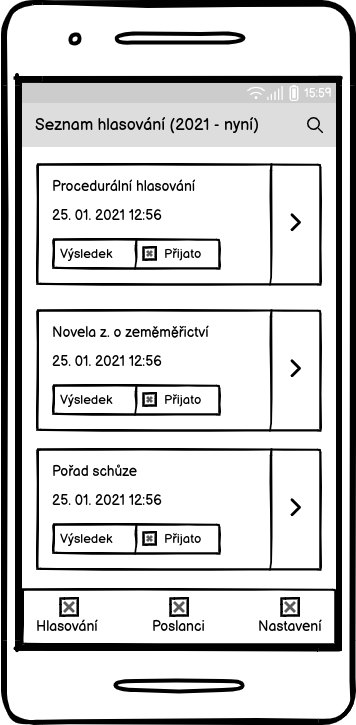
\includegraphics[scale = 0.5]{vote_list.png}
		\caption{Seznam hlasování}
		\label{fig:vote_list}
	\end{minipage}%
	\begin{minipage}{0.5\textwidth}
		\centering
		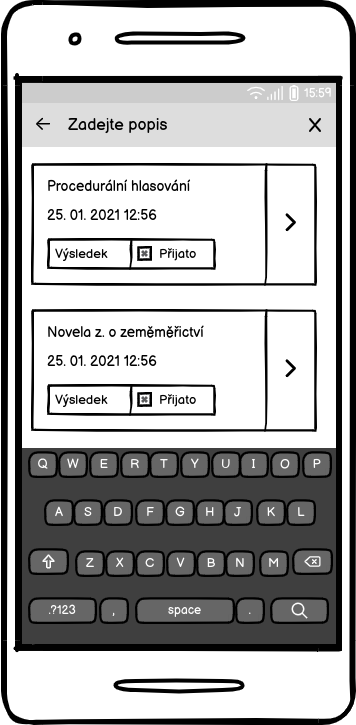
\includegraphics[scale = 0.5]{vote_list_search.png}
		\caption{Vyhledávání v seznamu hlasování}
		\label{fig:vote_list_search}
	\end{minipage}
	\caption{Obrazovka pro seznam hlasování}
\end{figure}

\begin{figure}[h]
	\begin{minipage}{0.5\textwidth}
		\centering
		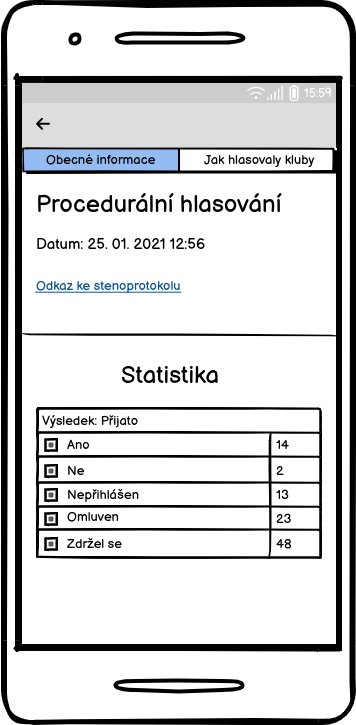
\includegraphics[scale = 0.4]{vote_details_general.png}
		\caption{Detail hlasování}
		\label{fig:vote_details_general}
	\end{minipage}%
	\begin{minipage}{0.5\textwidth}
		\centering
		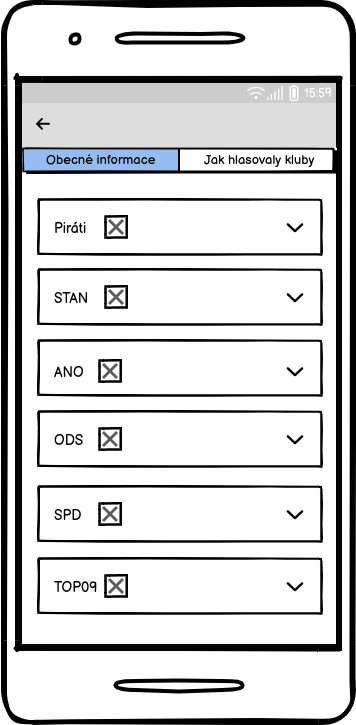
\includegraphics[scale = 0.4]{vote_details_party_votes.png}
		\caption{Jak hlasovaly kluby}
		\label{fig:vote_details_party_votes}
	\end{minipage}
	\begin{minipage}{0.5\textwidth}
	\centering
	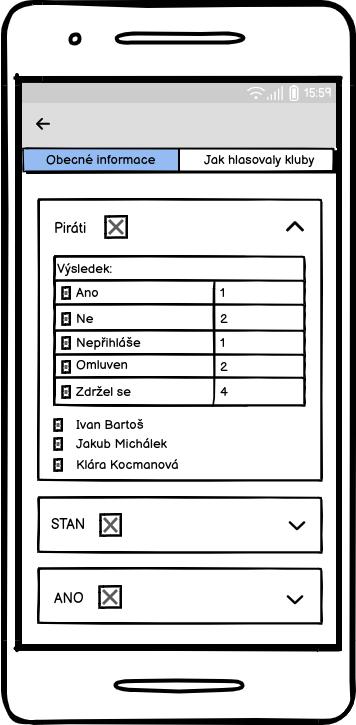
\includegraphics[scale = 0.4]{vote_details_party_votes_expanded.png}
	\caption{Jak hlasovaly kluby}
	\label{fig:vote_details_party_votes_expanded}
\end{minipage}
	\caption{Obrazovky pro detail hlasování}
\end{figure}

\begin{figure}[h]
	\begin{minipage}{0.5\textwidth}
		\centering
		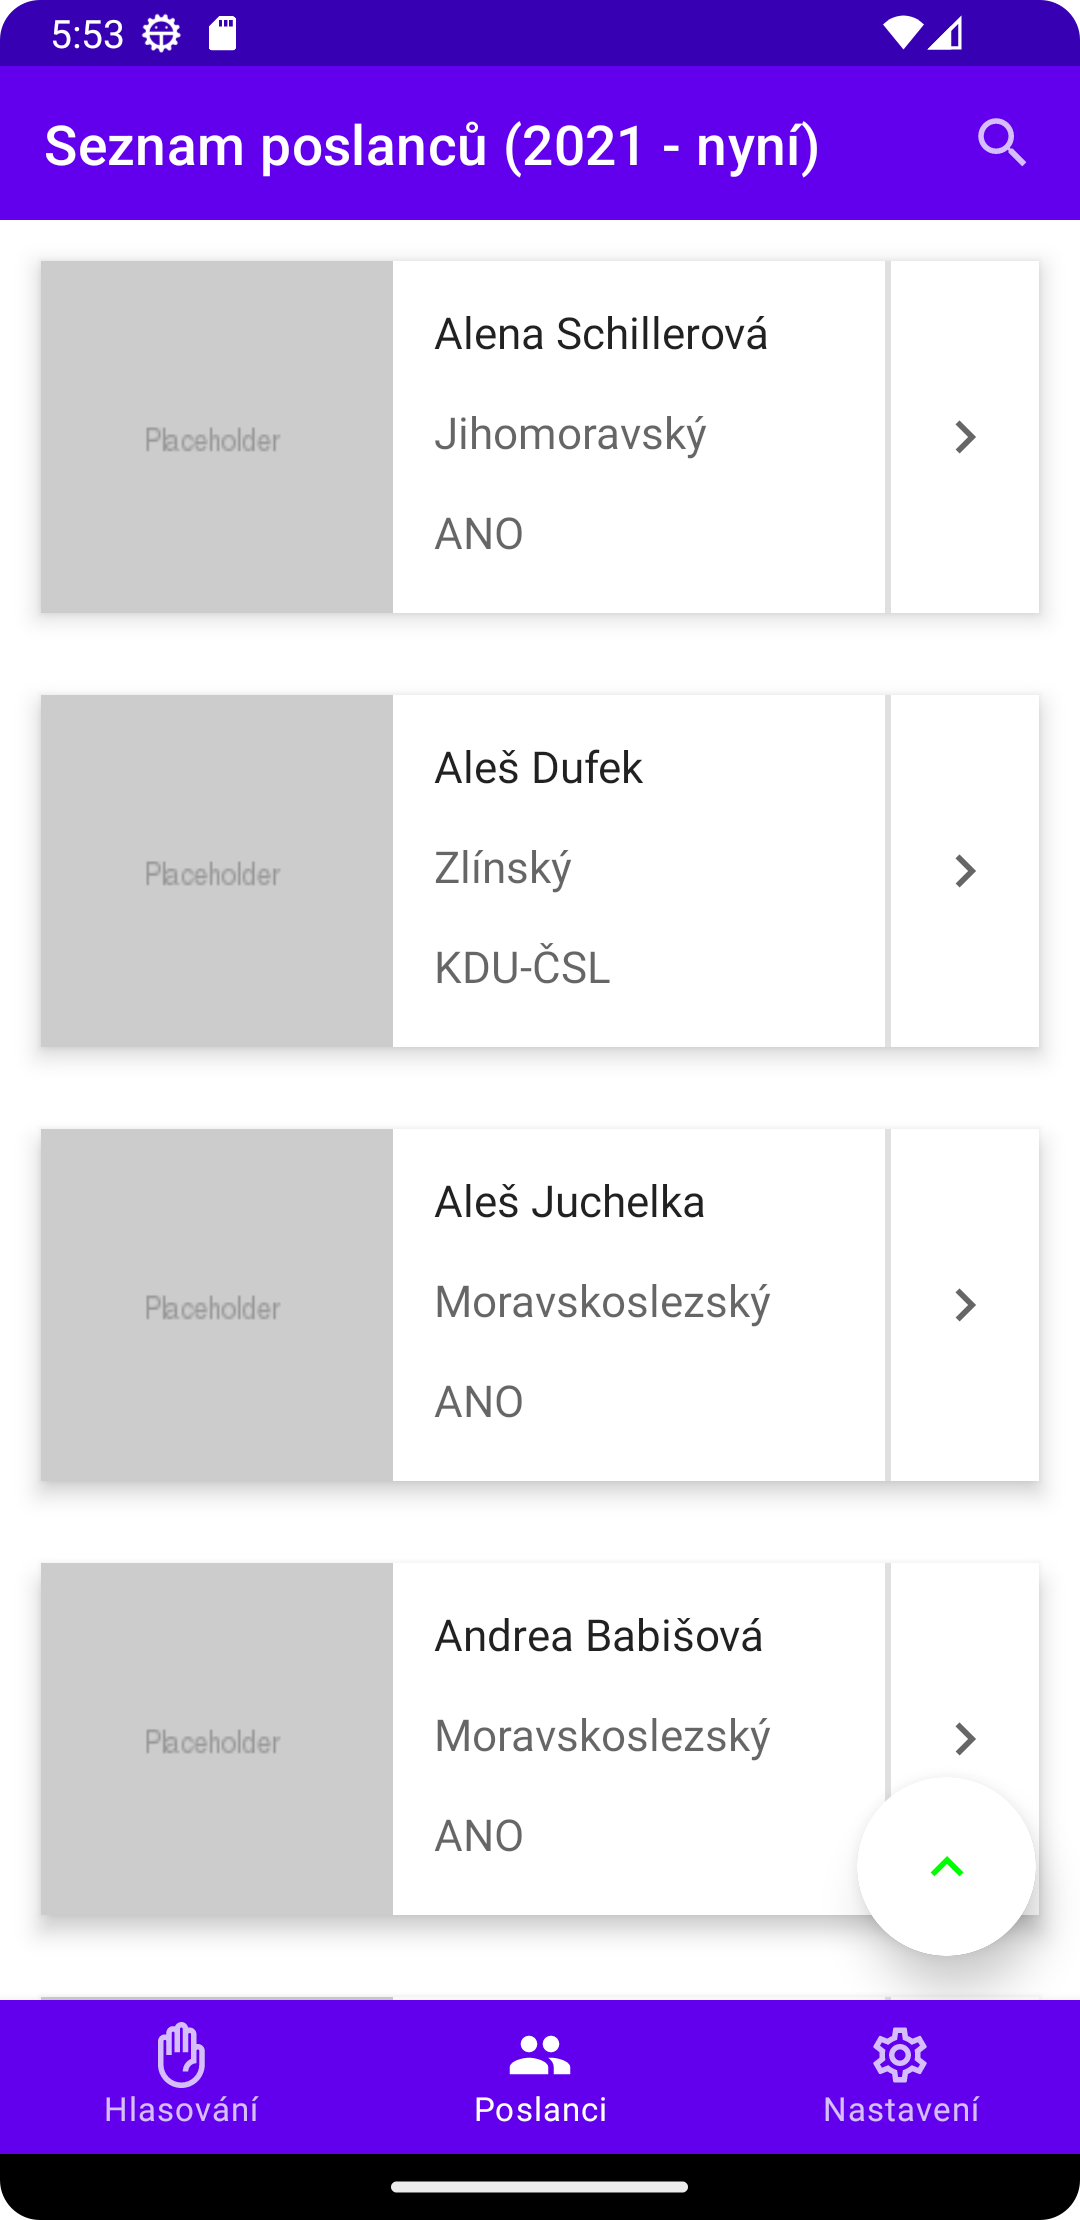
\includegraphics[scale = 0.5]{member_list.png}
		\caption{Seznam poslanců}
		\label{fig:member_list}
	\end{minipage}%
	\begin{minipage}{0.5\textwidth}
		\centering
		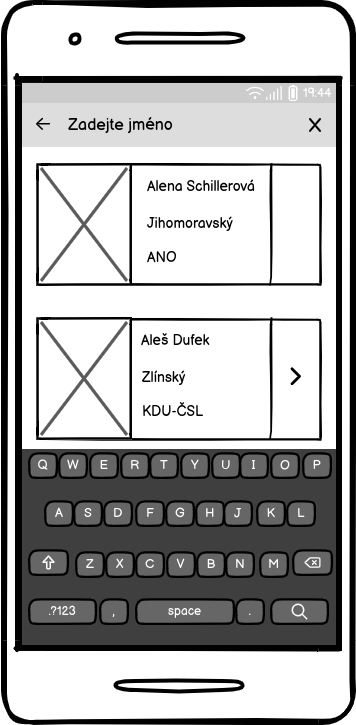
\includegraphics[scale = 0.5]{member_list_search.png}
		\caption{Vyhledávání v seznamu poslanců}
		\label{fig:member_list_search}
	\end{minipage}
	\caption{Obrazovka pro seznam poslanců}
\end{figure}

\begin{figure}[h]
	\begin{minipage}{0.5\textwidth}
		\centering
		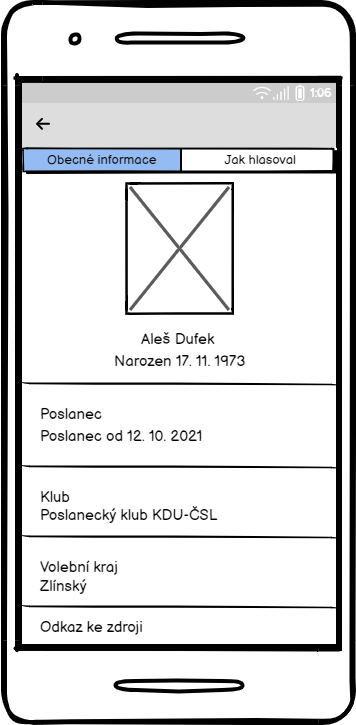
\includegraphics[scale = 0.5]{member_details_general.png}
		\caption{Detail poslance}
		\label{fig:member_details_general}
	\end{minipage}%
	\begin{minipage}{0.5\textwidth}
		\centering
		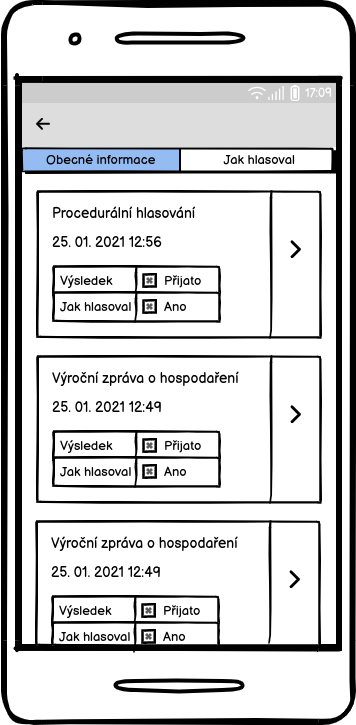
\includegraphics[scale = 0.5]{member_details_votes.png}
		\caption{Jak hlasoval/a poslanec/kyně}
		\label{fig:member_details_votes}
	\end{minipage}
	\caption{Obrazovky pro detail poslance}
\end{figure}

\begin{figure}[h]
	\begin{minipage}{0.5\textwidth}
		\centering
		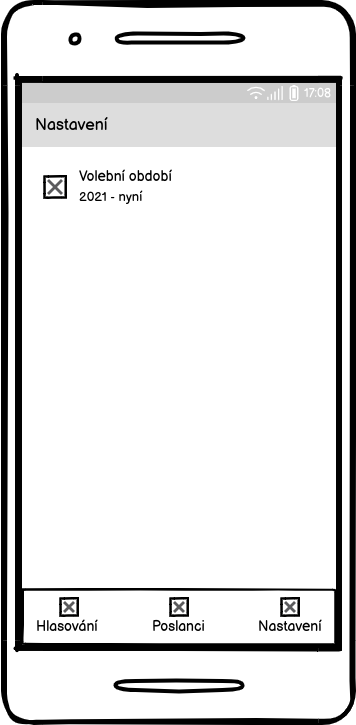
\includegraphics[scale = 0.5]{settings.png}
		\caption{Seznam nastavení}
		\label{fig:settings}
	\end{minipage}%
	\begin{minipage}{0.5\textwidth}
		\centering
		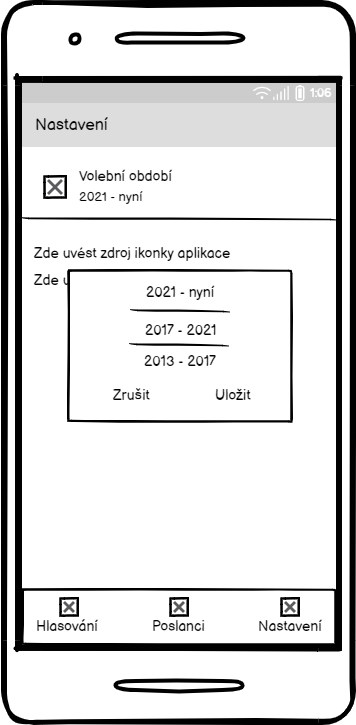
\includegraphics[scale = 0.5]{settings_opened.png}
		\caption{Nastavení volebního období}
		\label{fig:settings_opened}
	\end{minipage}
	\caption{Obrazovka pro nastavení}
\end{figure}

\begin{lstlisting}[caption={Tělo odpovědi pro dotaz \lstinline{GET /api/app}.}, label={fig:app}, language=json,firstnumber=1,tabsize=2]
{
	"election_years": [
	2021,
	2017,
	2013,
	2010,
	2006,
	2002,
	1998,
	1996,
	1992
	]
}
\end{lstlisting}

\begin{lstlisting}[caption={Tělo odpovědi pro dotaz \lstinline{GET /api/vote}}, label={fig:vote}, language=json,firstnumber=1,tabsize=2]
[
	{
		"id": 1,
		"date_time": "16. 12. 2022 13:29",
		"description": "Hlasovani 1",
		"result": "A"
	},
	{
		"id": 2,
		"date_time": "16. 12. 2022 13:26",
		"description": "Hlasovani 2",
		"result": "A"
	},
]
\end{lstlisting}

\begin{lstlisting}[caption={Tělo odpovědi pro dotaz \lstinline{GET /api/vote{id}}}, label={fig:vote-1}, language=json,firstnumber=1,tabsize=2]
{
	"id": 1,
	"date_time": "16. 12. 2022 13:29",
	"description": "Hlasovani 1,
	"result": "A",
	"steno_protocol_url": "http://www.psp.cz/eknih/2021ps/stenprot/048schuz/s048109.htm#h76",
	"yes_count": 100,
	"no_count": 0,
	"logged_off_count": 64,
	"excused_count": 0,
	"refrained_count": 36,
	"election_year": 0
}
\end{lstlisting}

\begin{lstlisting}[caption={Tělo odpovědi pro dotaz \lstinline{GET /api/party/vote/1}}, label={fig:party-vote-1}, language=json,firstnumber=1,tabsize=2]
[
	{
		"party_name": "Nazev klubu",
		"logo_url": "https://www.psp.cz/pics/klub/l-cps.jpg",
		"vote_id": 1,
		"party_results": {
			"yes_count": 2,
			"no_count": 0,
			"logged_off_count": 1,
			"excused_count": 0,
			"refrained_count": 0
		},
		"member_results": [
			{
				"member_name": "Poslanec 1",
				"vote_result": "@"
			},
			{
				"member_name": "Poslanec 2",
				"vote_result": "C"
			},
			{
				"member_name": "Poslanec 3",
				"vote_result": "A"
			},
			{
				"member_name": "Poslanec 4",
				"vote_result": "A"
			}
		]
	}
]
\end{lstlisting}

\begin{lstlisting}[caption={Tělo odpovědi pro dotaz ¨}, label={fig:member}, language=json,firstnumber=1,tabsize=2]
[
	{
		"id": 1,
		"name": "Poslanec 1",
		"party": "ANO",
		"photo_url": "https://www.psp.cz/eknih/cdrom/2021ps/eknih/2021ps/poslanci/i6474.jpg",
		"election_region": "Volebni kraj 1",
		"election_year": 2021
	},
	{
		"id": 2,
		"name": "Poslanec 2",
		"party": "ODS",
		"photo_url": "https://www.psp.cz/eknih/cdrom/2021ps/eknih/2021ps/poslanci/i6804.jpg",
		"election_region": "Volebni kraj 2",
		"election_year": 2021
	},
]
\end{lstlisting}

\begin{lstlisting}[caption={Tělo odpovědi pro dotaz \lstinline{GET /api/member/1}}, label={fig:member-1}, language=json,firstnumber=1,tabsize=2]
{
	"id": 1,
	"name": "Poslanec 1",
	"gender": "M",
	"party": "Poslanecky klub",
	"member_from": "12. 10. 2021",
	"member_to": null,
	"date_of_birth": "25. 09. 1970",
	"election_region": "Volebni kraj 1",
	"photo_url": "https://www.psp.cz/eknih/cdrom/2021ps/eknih/2021ps/poslanci/i6474.jpg",
	"election_year": 2021
}
\end{lstlisting}

\begin{lstlisting}[caption={Tělo odpovědi pro dotaz \lstinline{GET /api/member/1/vote}}, label={fig:member-vote-1}, language=json,firstnumber=1,tabsize=2]
[
	{
		"vote": {
			"id": 1,
			"date_time": "16. 12. 2022 13:29",
			"description": "Hlasovani 1",
			"result": "A"
		},
		"how_member_voted": "@"
	},
	{
		"vote": {
			"id": 2,
			"date_time": "16. 12. 2022 13:26",
			"description": "Hlasovani 2",
			"result": "A"
		},
		"how_member_voted": "@"
	}
]
\end{lstlisting}